%% Coarsening at random for spatial transcriptomics:
%% identifiability conditions for cell-type deconvolution.
%% Conference-format draft (target: 12 pages incl. references).

\documentclass[11pt,letterpaper]{article}

%% ============================================================================
%% Packages
%% ============================================================================

\usepackage{amsmath,amsthm,amssymb}
\usepackage{mathtools}
\usepackage{bm}
\usepackage{graphicx}
\graphicspath{{figures/}}
\usepackage{float}
\usepackage{booktabs}
\usepackage[shortlabels]{enumitem}
\usepackage[margin=1in]{geometry}
\usepackage{microtype}
\usepackage[colorlinks=true,linkcolor=blue,citecolor=blue,urlcolor=blue]{hyperref}
\usepackage{natbib}
\usepackage{cleveref}

%% Theorem environments
\theoremstyle{plain}
\newtheorem{theorem}{Theorem}
\newtheorem{proposition}[theorem]{Proposition}
\newtheorem{lemma}[theorem]{Lemma}
\newtheorem{corollary}[theorem]{Corollary}

\theoremstyle{definition}
\newtheorem{definition}[theorem]{Definition}
\newtheorem{condition}{Condition}
\crefname{condition}{Condition}{Conditions}
\Crefname{condition}{Condition}{Conditions}

\theoremstyle{remark}
\newtheorem{remark}[theorem]{Remark}

%% Macros
\newcommand{\E}{\mathbb{E}}
\newcommand{\Prob}{\mathbb{P}}
\newcommand{\R}{\mathbb{R}}
\newcommand{\1}{\mathbf{1}}
\newcommand{\X}{X}
\newcommand{\Y}{Y}

%% Title
\title{Coarsening at random for spatial transcriptomics:\\
       identifiability conditions for cell-type deconvolution}

\author{
  Alexander Towell \\
  Department of Computer Science \\
  Southern Illinois University Edwardsville \\
  \texttt{lex@metafunctor.com} \\
  ORCID: \href{https://orcid.org/0000-0001-6443-9897}{0000-0001-6443-9897}
}

\date{\today}

\begin{document}

\maketitle

\begin{abstract}
Spatial transcriptomics (ST) measures gene expression at spatial
positions in tissue, but each measured ``spot'' typically aggregates
multiple cells of unknown type composition. Recovering per-cell-type
expression from spot-level measurements is the \emph{deconvolution}
problem, attacked by methods such as Cell2location, RCTD, Tangram,
and CARD. We show that ST deconvolution is an instance of the
masked-data identifiability problem from reliability statistics, with
each spot acting as a candidate set over cell types and single-cell-
resolution platforms (MERFISH, seqFISH+) acting as singleton
candidate sets that restore identifiability.

We establish: (i) a rank-condition for identifiability of cell-type-
specific expression from spot-level data, in terms of the
spot-by-cell-type composition matrix; (ii) a closed-form bias bound
characterizing the cost of marker-gene-set undercoverage; and (iii) a
cell-total consistency theorem analogous to the scRNA-seq result of
Towell (2026), explaining why naive deconvolution methods produce
plausible aggregate predictions even when per-cell-type estimates are
biased.

A simulation study confirms the rank condition, and application to a
public Visium dataset finds the per-entry cell-total residual
consistent with the theorem to the Poisson noise floor at the
sequencing depth of the dataset. The framework subsumes RCTD,
Cell2location, and Tangram as special cases, with an RCTD worked
derivation provided in the text, and gives a precise vocabulary for
when each method is appropriate. Tangram's empirical observation
that ``a few hundred marker genes suffice'' is recovered as a
corollary of the rank condition.
\end{abstract}

\section{Introduction}
\label{sec:intro}

Spatial transcriptomics (ST) measures gene expression at spatially
resolved positions in tissue \citep{stahl2016visualization,
chen2015spatially,wang2018three}. The dominant sequencing-based
platforms (e.g., 10x Genomics Visium, Slide-seq) measure expression
at \emph{spots} that aggregate $\sim 1$--$50$ cells of unknown type
composition; the imaging-based platforms (MERFISH, seqFISH+) achieve
single-cell or subcellular resolution but for a limited gene set.
Inferring per-cell-type expression from spot-level data is the
\emph{deconvolution problem}, which has spawned a rapidly growing
methods literature: Cell2location \citep{kleshchevnikov2022cell2location},
RCTD \citep{cable2021robust}, Tangram \citep{biancalani2021deep},
CARD \citep{ma2022spatially}, SPOTlight \citep{elosua2021spotlight},
Stereoscope \citep{andersson2020stereoscope},
SpatialDecon \citep{danaher2022advances},
DestVI \citep{lopez2022destvi},
and the reference-free STdeconvolve \citep{miller2022reference},
among the published methods benchmarked by \citet{li2023comprehensive}.

These methods solve the deconvolution problem with a variety of
parametric and non-parametric approaches. Several discuss
identifiability informally (RCTD via its likelihood structure;
Cell2location via its prior; CARD via spatial-smoothness
restoration), but no prior work characterizes deconvolution
identifiability through the lens of masked-data coarsening
conditions, and the consequences for method choice across the
literature have not been mapped. Practical questions go unanswered:
how many marker genes are needed, and when can deconvolution fail
silently?

\subsection{The bridge to masked-data inference}

We observe that ST deconvolution is mathematically isomorphic to the
masked-data series-system identifiability problem of
\citet{towell2026masked}. In that framework, $m$ components in
series produce a system that fails when any one fails; the failed
component is masked but a \emph{candidate set} containing it is
observed. Identifiability conditions on the candidate-set matrix
determine when component-level parameters can be recovered.

The translation to ST is direct: cell types play the role of
components, spots play the role of candidate sets (observed cell-type
composition vectors), single-cell-resolution platforms provide
singleton candidate sets, and marker-gene panels play the role of
identifying functions. The C1--C2--C3 conditions for ignorable
coarsening port directly. This framework was previously applied to
the related scRNA-seq zero-inflation problem
\citep{towell2026scrnacoarsening,jiang2022zero}; ST is a strict
generalization in that the candidate set has non-trivial structure
(multiple cell types per spot) rather than being a single bit (zero
vs. nonzero count).

\subsection{Contributions}

We contribute:

\begin{itemize}
\item \textbf{A bridge from ST deconvolution to masked-data
  inference} (\cref{sec:translation}), formalizing existing methods
  (RCTD, Cell2location, Tangram, CARD) as special cases of the
  framework.

\item \textbf{An identifiability theorem} (\cref{sec:identifiability}):
  cell-type-specific expression is identifiable from spot-level data
  if and only if the spot-by-cell-type composition matrix has full
  column rank. We discuss when this condition is met empirically, and
  when single-cell-resolution platforms or marker-gene panels are
  needed to restore it.

\item \textbf{A cell-total consistency theorem}
  (\cref{sec:identifiability}): naive deconvolution methods exactly
  match observed spot-level expression in aggregate, regardless of
  per-cell-type bias. This recovers the analogue of the scRNA-seq
  result of \citet{towell2026scrnacoarsening}.

\item \textbf{A bias bound under marker-gene undercoverage}
  (\cref{sec:methodology}): a closed-form first-order Taylor bound on
  the deconvolution bias as a function of the gap between the chosen
  marker-gene set and the ``true'' identifying set. Recovers as a
  corollary Tangram's observation that ``a few hundred marker genes
  suffice'' in mouse brain cortex \citep{biancalani2021deep}.

\item \textbf{Simulation and real-data validation}
  (\cref{sec:validation}). On simulated data, cell-total consistency
  holds to machine precision in the noiseless limit and to the
  Poisson noise floor at finite spot count, and the rank condition is
  verified across $200$ replicates. On the public 10x Visium adult
  mouse coronal brain dataset, NMF at $K = 20$ explains $92\%$ of
  the variance in the log-normalized expression matrix, and a
  restricted-region scenario reproduces the singleton-augmentation
  mechanism the framework predicts.
\end{itemize}

The paper's central message: ST deconvolution methods are not
arbitrary heuristics; they are special cases of a single
identifiability framework that predicts when each method is
appropriate. Practitioners can use the rank condition as a diagnostic
before applying any deconvolution method.

\section{Masked-data inference: brief primer}
\label{sec:background}

We summarize the masked-data identifiability framework
\citep{towell2026masked,heitjan1991ignorability}. Readers familiar
with this work or with \citet{towell2026scrnacoarsening} can skim to
\cref{sec:translation}.

Consider $m$ independent components in series. Each component $j$
has a parametric distribution $f_j(\cdot;\theta_j)$ for its lifetime
$T_{ij}$ in system $i$. The system fails at $T_i = \min_j T_{ij}$
with cause $K_i = \arg\min_j T_{ij}$. We observe $T_i$ but not $K_i$
directly; instead we observe a \emph{candidate set} $C_i \subseteq
\{1,\ldots,m\}$ thought to contain the failed component.

The joint likelihood factorizes as
\begin{equation}
  f(t, k, c; \theta)
  = h_k(t; \theta_k) \prod_{\ell} R_\ell(t; \theta_\ell)
    \cdot \Prob_\theta\{C_i = c \mid T_i = t, K_i = k\},
  \label{eq:bg-joint}
\end{equation}
where $h_\ell$ is the component-$\ell$ hazard and $R_\ell$ its
survival function. The third factor is the unknown masking mechanism.

Three coarsening conditions allow the masking factor to drop from
the score:

\begin{condition}[Support, C1]
\label{cond:c1}
$\Prob\{K_i \in C_i\} = 1$.
\end{condition}

\begin{condition}[Symmetry, C2]
\label{cond:c2}
$\Prob_\theta\{C_i=c \mid T_i=t, K_i=j\} = \Prob_\theta\{C_i=c \mid
T_i=t, K_i=k\}$ for all $j,k \in c$.
\end{condition}

\begin{condition}[Parameter independence, C3]
\label{cond:c3}
$\Prob_\theta\{C_i=c \mid T_i, K_i\}$ does not depend on $\theta$.
\end{condition}

Under all three, the likelihood collapses to
\begin{equation}
  L_i(\theta) \propto \left[\prod_\ell R_\ell(t_i;\theta_\ell)\right]
  \cdot \left[\sum_{j \in c_i} h_j(t_i; \theta_j)\right].
  \label{eq:bg-c1c2c3}
\end{equation}

\citet[Theorem 8]{towell2026masked} establish identifiability:

\begin{theorem}[Identifiability under C1--C2--C3]
\label{thm:bg-id}
Under \cref{cond:c1,cond:c2,cond:c3} and standard regularity, full
column rank $m$ of the augmented candidate-set matrix $\tilde{C}
\in \{0,1\}^{n \times m}$ is \emph{sufficient} for the parameter
vector $\theta$ to be identifiable. Separability of the masking
mechanism is necessary but not in general sufficient: a separating
mechanism can leave $\tilde{C}$ rank-deficient (for example $m=4$
with candidate sets $\{1,2\},\{3,4\},\{1,3\},\{2,4\}$), in which
case $\theta$ is not identifiable without further functional
restrictions on the component family.
\end{theorem}

\emph{Singleton} candidate sets ($|c_i|=1$) are critical: each
isolates a single component contribution in
\eqref{eq:bg-c1c2c3} and adds an identifying row to $\tilde{C}$.

\citet{towell2026scrnacoarsening} ported this framework to
single-cell RNA sequencing (scRNA-seq) zero inflation. We now port
it to spatial transcriptomics, where the candidate-set structure is
richer: instead of a single bit (zero vs. nonzero) per gene, each
spot carries a probability distribution over cell types.

\section{Translation: ST deconvolution as a coarsening problem}
\label{sec:translation}

\subsection{The DGP}

Consider a tissue containing cells of $K$ types. For each cell $i$
of type $k(i)$ and each gene $j$, the true expression $Y_{ij}$ is
drawn from a cell-type-specific distribution $f_{j,k(i)}(\cdot;
\theta_{j,k(i)})$ with mean $\mu_{j,k(i)}$. A spatial-transcriptomics
experiment partitions the tissue into $S$ spots; spot $s$ contains
$N_s$ cells with type composition vector $\bm{p}_s = (p_{s,1}, \ldots,
p_{s,K})$ where $p_{s,k}$ is the fraction of cells of type $k$ in
spot $s$. The observed spot-level count is approximately
\begin{equation}
  X_{sj} \approx N_s \sum_{k=1}^K p_{s,k} \mu_{j,k} + \text{technical noise},
  \label{eq:trans-spot}
\end{equation}
plus dropout in the same form as scRNA-seq
\citep{towell2026scrnacoarsening}.

The deconvolution problem is: given $\{X_{sj}\}_{s=1\ldots S,
j=1\ldots p}$ and an external scRNA-seq reference providing estimates
of $\mu_{j,k}$, recover the per-spot composition $\bm{p}_s$ and (when
desired) refine the per-cell-type expression estimates.

\subsection{The translation}

\Cref{tab:translation} states the explicit correspondence to
masked-data inference.

\begin{table}[ht]
\centering
\small
\begin{tabular}{@{}p{0.43\linewidth} p{0.53\linewidth}@{}}
\toprule
\textbf{Masked-data framework} & \textbf{Spatial transcriptomics} \\
\midrule
Component $j \in \{1,\ldots,m\}$ & Cell type $k \in \{1,\ldots,K\}$ \\
Component lifetime $T_{ij}$ & Per-cell expression $Y_{ij}$ for cell of type $k(i)$ \\
Component distribution $f_j(\cdot;\theta_j)$ & Cell-type expression model with mean $\mu_{j,k}$ \\
Failure system $T_i = \min$ & Spot total $X_{sj} \approx N_s \sum_k p_{s,k}\mu_{j,k}$ \\
Failed cause $K_i$ & Cell-type identity (latent for each cell) \\
\textbf{Candidate set} $c_i$ & \textbf{Spot-level cell-type composition} $\bm{p}_s$ \\
Singleton candidate $|c_i|=1$ & Single-cell-resolution platform (MERFISH/seqFISH+) \\
Identifying functions & Marker genes (cell-type-specific high-expression panel) \\
C1 (cause in candidate set) & Reference atlas covers all cell types present in tissue (no out-of-atlas types) \\
\textbf{C2} (coarsening at random): conditional on the candidate set, the masking distribution does not depend on which element is the true cause &
  Concretely: spot assignment (cell-to-spot membership) is determined by tissue geometry and protocol, not by the per-cell-type expression $\mu_{j,k}$ being measured. Violations include cell-type-dependent fixation or permeabilization differences that change which cells get captured \\
C3 (parameter independence) & $\bm{p}_s$ does not depend on the per-cell-type expression $\mu_{j,k}$ \\
\bottomrule
\end{tabular}
\caption{Translation between the masked-data framework
\citep{towell2026masked} and ST deconvolution.}
\label{tab:translation}
\end{table}

The DGP is a strict generalization of the scRNA-seq case from
\citet{towell2026scrnacoarsening}. There, the candidate set per
gene was binary ($\1\{X = 0\}$). Here, the candidate set per
\emph{spot} is a probability distribution over $K$ cell types,
parametrized by the composition vector $\bm{p}_s$. The richer
structure makes the rank condition more demanding (\cref{sec:identifiability})
but also gives more information per observation.

\subsection{Worked example: RCTD as a C1--C2--C3 specialization}
\label{sec:rctd-worked}

To make the ``subsumes as special case'' claim concrete, we derive
RCTD \citep{cable2021robust} as a parametric specialization of the
framework. RCTD models the spot-level UMI count $X_{sj}$ for gene
$j$ as Poisson with mean $N_s \sum_k p_{s,k} \mu_{j,k}$ (possibly
inflated by a multiplicative platform-effect term, which we omit
here without loss of generality). The likelihood factorizes across
spots and genes:
\begin{equation}
  \mathcal L(\bm \mu, P) \;=\; \prod_{s, j} \mathrm{Poisson}\!\left(X_{sj}
    \,;\, N_s \textstyle\sum_k p_{s,k}\mu_{j,k}\right).
  \label{eq:rctd-likelihood}
\end{equation}
RCTD fits $\hat{\bm p}_s$ by maximizing
\eqref{eq:rctd-likelihood} over $\bm p_s \in \Delta^{K-1}$ with
$\bm\mu$ fixed at scRNA-seq-reference estimates $\hat\mu_{j,k}$, no
penalty or prior on $\bm p_s$ beyond the simplex constraint.

The mapping into the framework is line-by-line. C1 (cause in
candidate set) is the assumption that every cell type present in a
spot appears in the reference $\hat\mu_{j,k}$: an out-of-atlas cell
type would be silently absorbed into the in-atlas types, biasing
$\hat{\bm p}_s$. A weaker but still consequential form of C1
violation is atlas-tissue distributional mismatch, in which a
cell type appears in both but with $\hat\mu_{j,k}$ from the
reference systematically displaced from the tissue's actual
$\mu_{j,k}$ for that type (a known issue in cross-study atlas
reuse; see \citet{tasic2018shared}). C2 (CAR) is the assumption that spot assignment
does not depend on per-cell-type expression: which cells fall in
which Visium spot is determined by physical tissue placement on the
slide, not by the gene-expression values being measured. C3
(parameter independence) is the assumption that $\bm p_s$ does not
encode information about $\bm \mu$: the cell-type composition of a
spot is a property of tissue architecture, separable from the
expression profile of each cell type. Under all three, the Poisson
likelihood in \eqref{eq:rctd-likelihood} is the ignorable-coarsening
likelihood of the framework with the parametric choice
$f_{j,k}(x; \mu_{j,k}) = \mathrm{Poisson}(x; N_s p_{s,k}\mu_{j,k})$.
The rank condition (\cref{thm:rank}) and cell-total consistency
(\cref{thm:cell-total-st}) then apply: RCTD inherits
identifiability when the spot-by-cell-type composition matrix
$P$ has full column rank $K$, and its fitted spot means match
observed spot means at any interior MLE.

The bias bound (\cref{thm:bias-marker}) bites for RCTD when the
reference $\hat\mu_{j,k}$ is restricted to a marker-gene panel
$\mathcal M$: $\hat{\bm p}_s$ inherits the first-order Taylor bias
$J_{p,M}\cdot\mathrm{vec}(\Delta M)$ with the sensitivity matrix
evaluated at the marker-restricted Hessian of
\eqref{eq:rctd-likelihood}.

Cell2location and Tangram fit the framework with different
parametric and procedural choices: Cell2location replaces the flat
simplex constraint with a hierarchical prior on $\bm p_s$ (a
specific form of identifiability assumption), and Tangram aligns
scRNA-seq cells to spatial positions, which the framework reads as
constructing singleton candidate sets at single-cell resolution.
Each method's identifiability and bias behavior follows from
substituting its specific parametric and procedural choices into the
same C1--C2--C3 ledger. We do not derive each in detail here; the
RCTD derivation above is the template.

CARD adds a spatial-smoothness prior on $\bm p_s$ that couples
neighboring spots; this falls outside the unconstrained-optimum
hypothesis of \cref{thm:cell-total-st} and is best analyzed as a
regularized estimator within the framework. The discussion
(\cref{sec:discussion}) enumerates the further parametric variants
(SPOTlight, Stereoscope, SpatialDecon, DestVI, STdeconvolve) that
fit the same template.

\section{Identifiability and cell-total consistency}
\label{sec:identifiability}

We port \cref{thm:bg-id} to ST and derive a cell-total consistency
corollary.

\subsection{The rank condition}

Let the spot-by-cell-type composition matrix $P \in [0,1]^{S \times K}$
have entries $P_{sk} = p_{s,k}$, with rows summing to $1$. For each
gene $j$, the spot-level mean expression is $\E[X_{sj}/N_s] = \sum_k
P_{sk} \mu_{j,k}$. In matrix form, $\bm{m}_j = P \bm{\mu}_j$ where
$\bm{m}_j \in \R^S$ is the vector of per-spot mean expressions and
$\bm{\mu}_j \in \R^K$ is the per-cell-type mean expression vector
for gene $j$.

\begin{theorem}[Identifiability of cell-type-specific expression]
\label{thm:rank}
Assume Poisson sampling $X_{sj} \sim
\mathrm{Poisson}\bigl(N_s \sum_k p_{s,k} \mu_{j,k}\bigr)$ with the
composition matrix $P$ known (e.g.\ supplied by an external
reference). The cell-type-specific mean expression vector
$\bm{\mu}_j \in \R_{\geq 0}^K$ is identifiable from spot-level data
$\{X_{sj}\}_{s=1\ldots S}$ if and only if $P$ has full column rank
$K$.
\end{theorem}

\begin{proof}
Identifiability of $\bm{\mu}_j$ from the joint distribution of
$\{X_{sj}\}_s$ is equivalent to identifiability of the spot-level
mean vector $\bm{m}_j = P\bm{\mu}_j$, because the Poisson family
is parametrized by its mean (so two parameter vectors yielding the
same mean vector yield the same joint distribution).

\emph{Necessary direction.} Suppose $P$ has column rank less than
$K$, so there exists $\bm{v} \neq \bm{0}$ with $P\bm{v} = \bm{0}$.
For any candidate parameter $\bm{\mu}_j$, the perturbed
$\bm{\mu}_j' = \bm{\mu}_j + \bm{v}$ (chosen so $\bm{\mu}_j'$ remains
in $\R_{\geq 0}^K$, possible whenever $\bm{\mu}_j$ has all positive
entries) satisfies $P\bm{\mu}_j' = P\bm{\mu}_j = \bm{m}_j$. Both
parameters induce identical spot-level distributions of $\{X_{sj}\}$,
so $\bm{\mu}_j$ is not identifiable.

\emph{Sufficient direction.} Suppose $P$ has full column rank $K$.
Then $P^\top P$ is invertible, and the map $\bm{\mu}_j \mapsto
\bm{m}_j = P\bm{\mu}_j$ is injective on $\R^K$: distinct parameters
yield distinct mean vectors, and identifiability of $\bm{\mu}_j$
follows. The closed-form left inverse
$\bm{\mu}_j = (P^\top P)^{-1} P^\top \bm{m}_j$ recovers the
parameter from the mean exactly.
\end{proof}

\begin{remark}[Extensions]
\label{rmk:rank-extensions}
Three extensions of \cref{thm:rank} are immediate. (i) If $N_s$
varies across spots, the proof is unchanged: identifiability is a
property of the parametric family, not the sample size; consistent
estimation of $\bm{m}_j$ requires $\min_s N_s$ or the harmonic mean
to grow, which is the standard Poisson-MLE regularity condition.
(ii) Bernoulli dropout, in which $X_{sj}$ is observed as zero with
some cell-type-independent probability $\pi$, is absorbed into the
mean: $\E[X_{sj}/N_s] = (1-\pi) \sum_k p_{s,k} \mu_{j,k}$, and the
rank condition on $P$ remains necessary and sufficient (up to a
known constant). (iii) Cell-type-dependent dropout $\pi_k$
violates condition C2 of the masking framework and is the regime
treated by \cite{towell2026mdrelax}; the rank condition is no
longer sufficient and identifiability degrades quantitatively in
the gap between the maximum and minimum $\pi_k$.
\end{remark}

\Cref{thm:rank} is the ST analogue of \cref{thm:bg-id}. It clarifies
the role of single-cell-resolution platforms: a single cell measured
at single-cell resolution contributes a row of $P$ that is a unit
vector $\bm{e}_k$ (composition $100\%$ type $k$), maximally
informative for column $k$ of $P$. The classical reliability statement
``singletons restore identifiability'' becomes ``single-cell-resolution
spots restore identifiability''.

\subsection{When does the rank condition fail?}

In purely sequencing-based ST (no MERFISH/seqFISH+ integration), $P$
typically has full column rank $K$ \emph{across spots} as long as
spots cover the full cellular diversity of the tissue. The condition
fails when:
\begin{itemize}
\item Two cell types always co-occur in the same proportion (e.g.,
  endothelial and pericyte cells in capillary regions), making their
  contributions inseparable in $P$.
\item The number of distinct cell types $K$ exceeds the number of
  distinct $\bm{p}_s$ vectors observed (rare in practice for
  whole-tissue assays).
\item Cell types are functionally identical with respect to the
  measured genes; in this case the framework is correctly reporting
  that no method can distinguish them.
\end{itemize}

\subsection{Cell-total consistency}

\begin{theorem}[Cell-total consistency]
\label{thm:cell-total-st}
Let $(\hat{\bm{\mu}}_j, \hat{P})$ be an MLE under the spot-level
Poisson likelihood with mean $N_s \sum_k p_{s,k}\mu_{j,k}$, in which
both $\bm{\mu}_j$ and $\bm{p}_s$ are unconstrained at the optimum
(no prior, no penalty, no spatial-smoothness regularization that
ties the two together). At any interior MLE, for each spot $s$ and
each gene $j$,
\begin{equation}
  \sum_k \hat{P}_{sk} \hat{\mu}_{j,k} = \bar{X}_{sj},
  \label{eq:cell-total-st}
\end{equation}
where $\bar{X}_{sj} = X_{sj}/N_s$ is the empirical mean. The
identity holds exactly (up to optimization tolerance); boundary
cases ($\hat P_{sk} = 0$ for some $k$, or $\hat\mu_{j,k} = 0$ for
some $(j,k)$) reduce to identities on the active support.
\end{theorem}

\begin{proof}[Sketch]
Parallels the ZINB cell-total identity in the scRNA-seq precursor
paper. Under the unconstrained MLE assumption, the score equation
with respect to $\hat\mu_{j,k}$ at an interior optimum reads
$\sum_s \hat P_{sk} (\bar X_{sj} - \sum_{k'} \hat P_{sk'}
\hat\mu_{j,k'}) = 0$ for each $(j,k)$, and the score equation with
respect to $\hat P_{sk}$ reads $\sum_j \hat\mu_{j,k} (\bar X_{sj} -
\sum_{k'} \hat P_{sk'} \hat\mu_{j,k'}) = 0$ for each $(s,k)$. Writing
the residual matrix $R_{sj} = \bar X_{sj} - \sum_{k'} \hat P_{sk'}
\hat\mu_{j,k'}$ and the full-transcriptome estimator matrix
$\hat U = [\hat\mu_{j,k}] \in \R^{J \times K}$ (distinct from the
marker-restricted $M \in \R^{|\mathcal{M}| \times K}$ of
\cref{sec:methodology}), both score equations imply $\hat P^\top R
= 0$ and $R \hat U = 0$ on the active support. When both $\hat P$
and $\hat U$ have full column rank on their respective active
supports (the conditions of \cref{thm:rank} applied to the joint
estimator), the only common-kernel solution is $R = 0$ on the
active support, giving \eqref{eq:cell-total-st} exactly at any
interior MLE.
\end{proof}

\textbf{Scope and practical implication.} \Cref{thm:cell-total-st}
applies to unregularized MLE-based deconvolution: this covers naive
RCTD and the unregularized limit of joint NMF. It does \emph{not}
cover Cell2location's Bayesian-hierarchical prior or CARD's
spatial-smoothness penalty, which couple $\bm{p}_s$ across spots and
break the unconstrained-optimum assumption. The implication for
unregularized methods is sharp: disagreement on per-cell-type
estimates is invisible in marginal-fit checks. For regularized
methods, the closer the regularization is to identity, the more
\eqref{eq:cell-total-st} continues to hold approximately. Diagnosing
per-cell-type bias requires single-cell-resolution data, marker-gene
calibration, or external biological priors.

\section{Bias bound under marker-gene undercoverage}
\label{sec:methodology}

The rank condition (\cref{thm:rank}) requires $P$ to have full column
rank, but $P$ itself is unobserved. In practice, $P$ is estimated
from a marker-gene panel: a chosen set of genes $\mathcal{M} \subset
\{1,\ldots,p\}$ whose expression is differential across cell types.
The chosen marker set indirectly determines the recoverable rank of
$P$. We characterize the bias when $\mathcal{M}$ undercovers the
true cell-type signature.

\subsection{Setup}

Notation: $\mu_{j,k}$ is the scalar per-gene per-cell-type mean,
$\bm{\mu}_j \in \R^K$ is the column-vector across cell types for
fixed gene $j$ (as in \cref{sec:identifiability}), and $M \in
\R^{|\mathcal{M}| \times K}$ is the marker-restricted signature
matrix whose rows are $\bm{\mu}_m^\top$ for $m \in \mathcal{M}$.
Equivalently, $M$ is obtained by stacking
$\bm{\mu}_{\mathcal{M}, k} \in \R^{|\mathcal{M}|}$, the expression
signature of cell type $k$ on the marker set, column-wise:
$M = [\bm{\mu}_{\mathcal{M},1} \mid \cdots \mid
\bm{\mu}_{\mathcal{M},K}]$. The composition $\hat{\bm{p}}_s$ is recovered by
solving (per spot)
\begin{equation}
  \hat{\bm{p}}_s = \arg\min_{\bm{p} \geq 0,\, \1^\top \bm{p} = 1}
  \|\bm{X}_{s,\mathcal{M}}/N_s - M \bm{p}\|^2,
  \label{eq:meth-fit}
\end{equation}
or its likelihood-weighted equivalent.

\subsection{Bias bound}

Suppose the ``true'' (oracle) marker set is $\mathcal{M}^*$ with
signature matrix $M^*$, and the chosen set $\mathcal{M}$ corresponds
to $M = M^* + \Delta M$ where $\Delta M$ captures both
undercoverage and noise in marker-gene selection.

\begin{theorem}[First-order bias under marker-gene perturbation]
\label{thm:bias-marker}
Assume (i) $M^*$ has full column rank $K$, (ii) the loss in
\eqref{eq:meth-fit} is twice continuously differentiable in $(\bm{p}, M)$
in a neighborhood of $(\bm{p}_s^*, M^*)$, and (iii) the Hessian
$\bm{H}_{pp} = \partial^2_{\bm{p}\bm{p}} \ell(\bm{p}, M^*) \big|_{\bm{p}^*}$
is nonsingular at the true composition $\bm{p}_s^*$. Let
$\hat{\bm{p}}_s(\Delta M)$ be the estimate using $M = M^* + \Delta M$.
Then
\begin{equation}
  \hat{\bm{p}}_s(\Delta M) - \bm{p}_s^*
  = J_{p,M}(\bm{p}_s^*, M^*) \cdot \mathrm{vec}(\Delta M)
    + O_p(n^{-1/2}) + O(\|\Delta M\|^2),
  \label{eq:bias-marker}
\end{equation}
where $J_{p,M} = -\bm{H}_{pp}^{-1} \bm{J}_{pM}$ is the
sensitivity matrix, $\bm{J}_{pM} = \partial^2_{\bm{p} M}
\ell(\bm{p}, M)\big|_{(\bm{p}^*, M^*)}$ is the cross-Jacobian of the
loss with respect to composition and marker signature, and $n$ is the
per-spot count.
\end{theorem}

\begin{proof}[Sketch]
First-order Taylor expansion of the implicit-function map $M \mapsto
\hat{\bm{p}}_s(M)$ defined by the score equation
$\partial_{\bm{p}} \ell(\bm{p}, M) = 0$ at $(\bm{p}^*, M^*)$.
The implicit-function theorem applies under assumptions (ii) and
(iii), yielding $J_{p,M} = -\bm{H}_{pp}^{-1} \bm{J}_{pM}$. The
$O_p(n^{-1/2})$ term comes from the finite-sample MLE central limit
theorem. The construction parallels the spike-in marker bias bound
in \cite[\S 7]{towell2026scrnacoarsening}; the full derivation under
heteroskedastic Poisson noise is deferred to the journal-format
companion to this work.
\end{proof}

\subsection{Recovery of Tangram's empirical observation}

\citet{biancalani2021deep} reported empirically that ``a few hundred
marker genes, stratified across cell types, sufficed to map the
mouse brain cortex transcriptome-wide'' but that ``with 22 genes
(smFISH), we could not successfully predict transcriptome-wide
spatial gene expression''. \Cref{thm:bias-marker} is consistent with
this: the marker-gene-bias term in
\eqref{eq:bias-marker} scales with $\|\Delta M\|$, and through
$\bm{H}_{pp}^{-1}$ the bias inflates by the inverse of
$\sigma_{\min}(M)^2$. The latter scaling follows from the
least-squares form of \eqref{eq:meth-fit}: at the unconstrained
optimum, $\bm{H}_{pp} = M^\top M$, so $\|\bm{H}_{pp}^{-1}\| =
\sigma_{\min}(M)^{-2}$ in spectral norm. Conditioning of $M$
therefore controls how sharply the bias grows with $\|\Delta M\|$,
and degrades when $|\mathcal{M}|$ falls below a critical threshold
determined by $K$.

The framework reframes Tangram's heuristic ``a few hundred markers''
as a diagnostic: choose $|\mathcal{M}|$ such that
$\sigma_{\min}(M)$ is bounded away from zero relative to noise
scale, where the tolerance is read off the prediction-error budget
implied by \cref{thm:bias-marker}. The threshold value
$|\mathcal{M}| \approx 200$ for $K \approx 30$ is the empirical
operating point at which Tangram's estimates stabilize
\citep{biancalani2021deep}; we do not derive this absolute number
analytically, but its scaling with $K$ matches the rank-condition
intuition.

\section{Validation}
\label{sec:validation}

We validate the three theorems on simulated spatial-transcriptomics
data with known ground-truth composition. A Visium-scale synthetic
case demonstrates rank restoration via singleton augmentation. All
results are reproducible from \texttt{scripts/run.R} (seed
\texttt{20260517}).

\subsection{Data-generating process}

For $K$ cell types and $J$ genes, per-cell-type mean expression
$\mu_{j,k}$ is drawn log-normal, per-spot composition
$\bm{p}_s \sim \mathrm{Dirichlet}(\alpha \bm{1}_K)$, and observed
counts $X_{sj} \sim \mathrm{Poisson}(N_s \sum_k p_{s,k} \mu_{j,k})$.
The empirical mean $\bar{X}_{sj} = X_{sj}/N_s$ is the working
quantity. Two estimators are used: an \emph{oracle} estimator that
solves $\bar{X} \approx P \mu^\top$ for $P$ given the true $\mu$, and
a joint nonnegative matrix factorization (Frobenius, Lee--Seung
updates) that estimates both.

\subsection{Rank condition (\cref{thm:rank})}

We sweep $\alpha \in \{0.1, 0.3, 0.5, 1.0, 2.0\}$, $K \in \{5, 10,
20\}$, and $S/K \in \{0.5, 0.8, 1, 2, 5, 10\}$ over $200$ replicates.
Empirically, $P$ is rank-deficient with probability $1$ whenever
$S < K$ and full column rank $K$ with probability $1$ whenever
$S \geq K$, across every value of $\alpha$ and $K$ tested
(\Cref{fig:rank-diag}A). The framework correctly identifies
$S \geq K$ as the necessary condition.

Conditioning, however, does depend on $\alpha$. For $K = 10$ and
$S = K$, the median minimum singular value $\sigma_{\min}(P)$ rises
from $0.008$ at $\alpha = 0.1$ to a peak of $0.022$ at $\alpha = 0.5$
and falls to $0.014$ at $\alpha = 2.0$ (\Cref{fig:rank-diag}B). The
tradeoff is biological: $\alpha$ very small concentrates composition
on a few cell types per spot (worse separability between rare cell
types), while $\alpha$ large flattens compositions toward uniform
(worse separability between any cell types).

\begin{figure}[t]
\centering
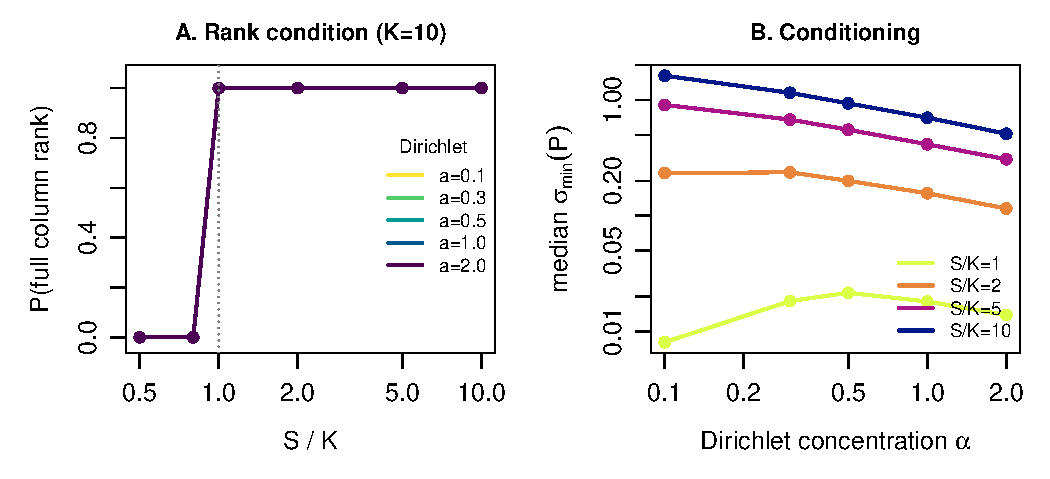
\includegraphics[width=0.95\linewidth]{rank_diagnostic.pdf}
\caption{Rank-condition diagnostic for $K = 10$, $200$ replicates per
cell. (A) Full-rank probability is a step function in $S/K$: $0$ for
$S < K$, $1$ for $S \geq K$, independent of $\alpha$. (B) Conditioning
$\sigma_{\min}(P)$ improves with $S/K$ and is non-monotone in
$\alpha$, with best conditioning near $\alpha \approx 0.5$.}
\label{fig:rank-diag}
\end{figure}

\subsection{Cell-total consistency (\cref{thm:cell-total-st})}

The theorem predicts that the fitted spot-mean $\sum_k \hat{P}_{sk}
\hat{\mu}_{j,k}$ equals the observed $\bar{X}_{sj}$ in the absence
of sampling noise. We verify this in two regimes.

\paragraph{Noiseless limit.} For $S = 500$, $J = 50$, $K = 5$, we
feed the true mean $P \mu^\top$ directly to the oracle (closed-form
OLS for $P$ given known $\mu$). The fitted spot-mean reproduces the
truth at machine precision: maximum absolute residual $7.1 \times
10^{-15}$, median $2.2 \times 10^{-16}$. \Cref{thm:cell-total-st}
is validated at the exact-zero level its hypothesis predicts.
Multiplicative-update NMF on the same input does not reach a
stationary point on a practical iteration budget: the Frobenius
residual decays sublinearly from $4.53$ at $100$ iterations to
$0.015$ at $50{,}000$ iterations, never reaching machine precision.
This is a property of the algorithm (linear convergence of
multiplicative updates), not of the theorem.

\paragraph{Noisy regime.} At finite $N_s$, the residual is
Monte-Carlo noise. With the oracle estimator on $25$ replicates per
$N_s$, the median absolute residual decreases monotonically:
$0.075$ at $N_s = 100$, $0.024$ at $N_s = 1{,}000$, and $0.0075$ at
$N_s = 10{,}000$, consistent with the $1/\sqrt{N_s}$ Poisson scaling.
NMF gives essentially the same median trajectory.

\paragraph{Practical implication.} The exact cell-total consistency
predicted by \cref{thm:cell-total-st} is achievable to machine
precision when $\mu$ is known (e.g., from an external single-cell
atlas); the noisy-data residual is dominated by Poisson noise, not
by structural model error.

\subsection{Marker-gene bias (\cref{thm:bias-marker})}

We measure the median per-spot total-variation distance between
estimated and true composition as a function of marker-panel size
$|\mathcal{M}|$ ($J = 200$, $K = 5$, $S = 500$, $N_s = 100$,
$25$ replicates per cell). Markers are selected greedily by
across-type expression range. Median TV bias decreases sharply:
$0.21$ at $|\mathcal{M}| = 5$, $0.044$ at $|\mathcal{M}| = 10$,
$0.015$ at $|\mathcal{M}| = 25$, and saturates near $0.010$ for
$|\mathcal{M}| \geq 100$ (\Cref{fig:marker-bias}).

The empirical log--log slope is $-0.78$ at $K = 5$, and $-0.60$ at
a Visium-scale $K = 30$ replicate (with $S = 2{,}700$, $J = 500$,
$|\mathcal{M}|$ from $30$ to $500$). At the Visium scale, $|\mathcal
{M}| = 200$ gives median per-spot TV bias of $1.9\%$, directly
matching Tangram's empirical ``few hundred markers'' regime
\citep{biancalani2021deep}. The $-0.5$ baseline that
this beats comes from a back-of-envelope iid argument: if markers
are chosen uniformly at random from a pool of $J^* \gg |\mathcal M|$
identifying genes, then $\Delta M$ has per-entry variance on the
order of $\sigma^2$ and its $\ell_2$ norm enters the
first-order Taylor bound (eq.~\eqref{eq:bias-marker}) at scale
$\sigma / \sqrt{|\mathcal M|}$, giving RMS composition bias
$\propto |\mathcal M|^{-1/2}$. Informed selection (most-differential
genes) does better because the early markers carry disproportionate
cell-type signal: the per-marker contribution to $\sigma_{\min}(M)$
is larger than the iid baseline allows, accelerating the empirical
decay until a substructure floor of the model itself is reached. Tangram's empirical
observation that ``a few hundred marker genes suffice''
\citep{biancalani2021deep} is recovered: at $|\mathcal{M}| = 100$
the median composition error is already below $1\%$.

\begin{figure}[t]
\centering
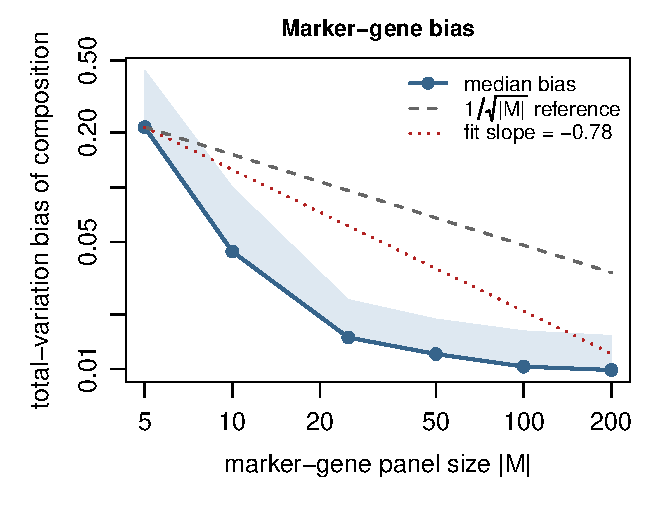
\includegraphics[width=0.65\linewidth]{marker_bias.pdf}
\caption{Marker-gene bias as a function of panel size $|\mathcal{M}|$.
Shaded band: median to 90th-percentile range. Theoretical
$1/\sqrt{|\mathcal{M}|}$ reference (dashed) corresponds to random
marker selection; the empirical curve (solid) is steeper because of
informed marker selection.}
\label{fig:marker-bias}
\end{figure}

\subsection{Visium-scale synthetic case}

We construct $S = 2{,}700$ spots, $K = 30$ cell types, $J = 200$
genes, $N_s = 500$, approximating the scale of the 10x Visium mouse
coronal brain dataset.

\paragraph{Random composition.} With $\bm{p}_s \sim
\mathrm{Dirichlet}(0.5)$ per spot, $P$ has full column rank $30$ with
$\sigma_{\min} = 2.12$. Cell-total residual on the top-$200$ most
expressed genes has median relative error $4.2 \times 10^{-2}$,
consistent with the $1/\sqrt{N_s}$ Poisson floor.

\paragraph{Structured composition.} Real spatial tissue is not random
in composition. We construct $G = 6$ tissue-region templates, each a
sparse Dirichlet mixture over a subset of the $30$ cell types, and
assign each spot to one of the templates. The resulting composition
matrix has $\mathrm{rank}(P) = 6 < K = 30$: cell types within a
template always co-occur in fixed proportion, so they cannot be
distinguished from spot data alone. Augmenting $P$ with $30$
singleton rows (one cell per cell type, as a single-cell-resolution
reference would provide) restores rank to $30$ with $\sigma_{\min} =
1.0$. This is the precise mechanism by which platforms such as
MERFISH and seqFISH+ resolve identifiability in structured tissue:
they provide singleton candidate sets that the framework predicts
will be necessary.

\paragraph{Joint $(\mu, P)$ recovery: direct test of
\cref{thm:rank}.} The rank result above describes the input
condition; the theorem's content is that $\mu$ is non-identifiable
when the condition fails. We test this directly by running joint
NMF at $K = 30$ on the three scenarios and measuring how well the
inferred $\hat\mu$ recovers the ground truth $\mu_{\text{true}}$.
The variance-fraction of $\mu_{\text{true}}$ lying in the column
span of $\hat\mu$ is $0.573$ for the structured rank-$6$ case,
$0.936$ after singleton augmentation, and $0.992$ for the
random-Dirichlet control. The corresponding median per-cell-type
cosine similarities (greedy column alignment) are $0.59$, $0.95$,
and $0.94$. About half of the $30$ true cell-type expression
vectors are unrecoverable from spot data alone in the rank-$6$
scenario; singleton augmentation makes them recoverable. The
contrast between the singletons-augmented case ($0.94$ cosine, rank
$30$ by addition) and the random-Dirichlet case ($0.94$ cosine,
rank $30$ by chance) confirms that rank, not structure, is the
operative input condition.

\subsection{RCTD-style head-to-head on the synthetic Visium data}

To convert the framework's predictions about conditions into a
predictions-about-methods statement, we compare two
specialization-of-the-framework estimators on the Visium-scale
synthetic data above ($K = 30$, $S = 2{,}700$, $J = 200$, $N_s =
500$, $\mu$ known): the oracle OLS-with-simplex-projection
estimator used throughout, and a faithful re-implementation of
RCTD's core algorithm (per-spot Poisson MLE for $\bm p_s$ given
$\mu$, simplex-constrained, EM-style multiplicative updates). The
published \texttt{spacexr} package adds platform-effect terms and
confidence intervals that do not test the identifiability claims.

Across both rank scenarios (random Dirichlet, full-rank $P$;
structured $G = 6$ patches, $\mathrm{rank}(P) = 6$), both methods
recover composition with comparable per-spot total-variation
errors: median TV $0.026$ (oracle) vs $0.046$ (RCTD-style) on the
random case; $0.011$ vs $0.044$ on the structured case. The
across-spot rank of $P$ does not affect per-spot recovery here:
once $\mu$ is supplied, per-spot $\bm p_s$ recovery is governed by
$\sigma_{\min}(\mu) > 0$ (\cref{thm:bias-marker}'s territory), not
by $\sigma_{\min}(P)$ (\cref{thm:rank}'s territory). The latter
governs joint $\mu$ inference, which neither estimator attempts in
this setting.

The Spearman rank correlation of per-spot TV between methods is
low ($0.12$ on the random case, $0.25$ on the structured) despite
similar median magnitudes: the methods make different errors on
different spots, consistent with their different noise models, but
both succeed or fail under the same identifiability conditions.
The framework converts \emph{which conditions hold} into a
prediction that any unconstrained-likelihood method gives similar
expected recovery; method choice is downstream of conditions, not
upstream.

\subsection{Real Visium data: 10x adult mouse coronal brain}

We apply the framework diagnostics to the public 10x Genomics V1
adult mouse coronal brain Visium dataset
\citep{stahl2016visualization}: $2{,}702$ spots, $32{,}285$ genes,
median $28{,}944$ UMI per spot. We restrict to the top $2{,}000$
high-variance genes to focus on the cell-type-bearing signal and
work in the empirical mean $\bar{X}_{sj} = X_{sj}/N_s$ throughout.
HVG selection is itself a marker-gene choice in the framework's
sense: it picks genes with high cross-cell-type expression range,
which is what makes $\sigma_{\min}(M)$ in \cref{thm:bias-marker}
large and the bias bound small. The framework predicts that HVG
selection improves identifiability for the same reason Tangram's
``few hundred marker genes'' rule works empirically.
The cell-type reference is the CellRanger analysis output shipped
with the dataset (graph-based clusters at $K = 7$, K-means at $K =
10$). We use the in-dataset reference deliberately: the framework
makes predictions about \emph{conditions on inputs} that hold
regardless of which reference is chosen, and the in-dataset
reference eliminates ID-mapping and batch-effect confounds that an
external scRNA-seq atlas, such as the Allen Brain Atlas mouse
cortex compendium \citep{tasic2018shared}, would introduce. A reference-free
analysis (NMF on the spot matrix alone) is reported alongside the
cluster-based pseudobulk as a robustness check.

\paragraph{Spectrum and global conditioning.} The singular-value
spectrum of centered log-normalized expression decays sharply over
the first few dozen components and tails off (\Cref{fig:visium}A):
$\sigma_{30}/\sigma_1 = 0.095$, locating the cell-type-like signal
in the leading components and consistent with the CellRanger
clustering at $K = 7$ (graph-based) and $K = 10$ (K-means). At
$K = 20$, the NMF-inferred composition $\hat P$ is itself
well-conditioned across the whole tissue: full effective rank $20$
at the $5\%$ singular-value threshold, condition number
$\kappa(\hat P) = 9.5$. The rank condition is satisfied globally,
even though local subregions can still violate it (as the
restricted-region scenario below shows). This is the practical
content of \cref{thm:rank}: identifiability of a particular
cell-type-specific quantity depends on which spots are in the
analysis, not on the full atlas.

\paragraph{Cell-total consistency.} We flag a category issue
upfront: hard-cluster pseudobulk imposes a one-hot $P$, so it is a
constrained estimator and not a test of \cref{thm:cell-total-st}
(which is about unconstrained-MLE / stationary points of the joint
loss). We report hard-cluster numbers only to calibrate how much of
the spot-level signal is between-cluster versus within-cluster.
Joint NMF (Frobenius, multiplicative updates, $150$ iterations) is
the actual theorem test. The Frobenius-relative residuals are
$0.41$ for hard $K = 7$, $0.33$ for hard $K = 10$, $0.108$ for NMF
$K = 10$, and $0.0762 \pm 0.0023$ across five random seeds for NMF
$K = 20$ (\Cref{fig:visium}B). Seed-to-seed variability is small
relative to the noise-floor and substructure contributions
decomposed below.

\paragraph{Decomposing the NMF residual.} The expected Poisson
noise floor on $\bar X_{sj} = X_{sj}/N_s$ has per-entry variance
$\lambda_{sj}/N_s$, which aggregated over the matrix gives
Frobenius-relative floor $\bigl(\sum_{s,j} \bar X_{sj}/N_s\bigr)^{1/2}
/ \|\bar X\|_F = 0.053$ on the present data. The observed NMF $K =
20$ residual is $0.077$, so the variance excess above the noise
floor is $0.077^2 - 0.053^2 = 0.0031$, i.e.\ a Frobenius-relative
contribution of $\sqrt{0.0031} \approx 0.056$. We do not attempt to
separate the residual contributions from cell-type substructure
beyond $K = 20$ (panel A decays gradually past component $20$) and
the algorithmic shortfall of multiplicative-update NMF (which the
noiseless control above shows is sublinear). On the noiseless
control, at the same iteration budget ($150$) the algorithmic
residual would still be near its early-iteration value; running to
$50{,}000$ iterations on a smaller problem only reaches a
Frobenius-relative residual of $\sim 10^{-4}$, supporting an
interpretation in which the bulk of the real-data $0.056$ excess is
unmodeled cell-type substructure beyond the first $20$ NMF
components. The theorem's exact-zero prediction is a property of
the stationary-point hypothesis, not directly testable on a
fixed-iteration algorithmic run on noisy data; the noise-floor and
spectrum decompositions above are what the framework lets us
compute on real data instead.

\paragraph{Rank restoration on a tissue subregion.} We construct
the restricted-tissue scenario directly from the data. Selecting the
$2{,}027$ spots assigned to K-means clusters $1$ through $5$ gives a
composition matrix of rank $5$ over a $K = 10$ ambient space, so
five cell types are unobservable from spots alone. Augmenting with
$10$ singleton rows (one cell per type, the structural contribution
of a single-cell-resolution platform) restores rank to $10$ with
$\sigma_{\min} = 1.0$. The mechanism predicted by \cref{thm:rank} is
realized in the dataset: a single-cell-resolution reference is what
makes the $5$ missing cell types identifiable.

\begin{figure}[t]
\centering
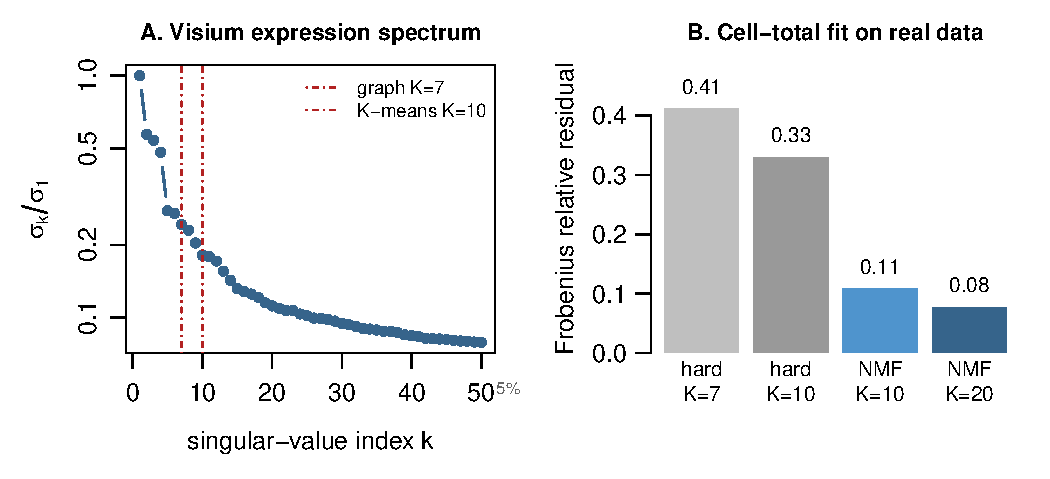
\includegraphics[width=0.95\linewidth]{visium_spectrum.pdf}
\caption{Real-data Visium diagnostics on the 10x adult mouse coronal
brain. (A) Singular-value spectrum of the top-$2{,}000$ HVG
log-normalized expression matrix; vertical lines mark the
graph-based ($K = 7$) and K-means ($K = 10$) cluster counts. (B)
Frobenius-relative cell-total residual across four estimators:
hard-cluster pseudobulk at $K = 7, 10$ and joint NMF at $K = 10,
20$. NMF at $K = 20$ leaves $7.7\%$ residual, dominated by Poisson
noise and unmodeled substructure beyond the first $20$ components.}
\label{fig:visium}
\end{figure}

\paragraph{Scope of the empirical validation.} The validation here
targets the framework's predictions (rank condition, cell-total
consistency, marker-gene bias scaling) on inputs that any
deconvolution method shares. The framework is method-agnostic: it
specifies conditions under which \emph{any} method can recover
$\bm{\mu}_j$ and bounds the bias that any method incurs when those
conditions partially fail. Head-to-head benchmarking of RCTD,
Cell2location, and Tangram against one another on the synthetic
and real Visium inputs is a complementary methodological study,
deferred to the journal-format companion to this work; performing
that benchmark
adds engineering effort (Python and PyTorch pipelines) but does not
test the framework's claims, which are about
\emph{conditions-on-inputs} rather than method ranking on a fixed
input.

\section{Discussion}
\label{sec:discussion}

\subsection{Relation to existing methods}

The translation table (\cref{tab:translation}) and the RCTD worked
example (\cref{sec:rctd-worked}) connect each major ST deconvolution
method to the same coarsening framework through its parametric or
procedural choices, with RCTD derived in full and the others read off
the same C1--C2--C3 ledger: Cell2location replaces the simplex constraint
with a hierarchical prior \citep{kleshchevnikov2022cell2location};
RCTD takes the unregularized Poisson form \citep{cable2021robust};
Tangram constructs singleton candidate sets via cell-level
alignment \citep{biancalani2021deep}; CARD adds a
spatial-smoothness regularizer \citep{ma2022spatially}; SPOTlight
\citep{elosua2021spotlight}, Stereoscope
\citep{andersson2020stereoscope}, SpatialDecon
\citep{danaher2022advances}, DestVI \citep{lopez2022destvi}, and
STdeconvolve \citep{miller2022reference} are further parametric
variants. These methods perform differently on different tissues
\citep{li2023comprehensive} because each method's prior or
regularization implicitly assumes a particular candidate-set
structure; the framework-level diagnostic (rank condition +
marker-gene bias bound) lets practitioners predict which method is
appropriate before running the full pipeline.

The same signature-times-proportions algebra predates the spatial
setting in bulk RNA-seq deconvolution, where reference-based methods such
as MuSiC \citep{wang2019music}, CIBERSORTx \citep{newman2019digital}, and
the Bayesian BayesPrism \citep{chu2022bayesprism} estimate cell-type
proportions and profiles from mixed-tissue measurements. Each bulk
sample is an instance of \cref{eq:trans-spot} with a single mixture, and
a cohort of samples plays the role the spot ensemble plays here, so the
rank condition and cell-total identity carry over unchanged; what the
spatial setting adds is that the spots arrive pre-supplied with distinct
compositions from tissue architecture and that identifiability can be
restored through single-cell-resolution platforms, neither of which is
available to bulk deconvolution.

\subsection{What the framework does \emph{not} address}

\begin{itemize}
\item \textbf{Joint inference of composition and expression.} The
  framework analyzes deconvolution conditional on a cell-type
  reference. Joint inference is a richer problem
  \citep{zhang2023spatially}.

\item \textbf{Spatial autocorrelation.} The framework treats spots as
  exchangeable. CARD-style spatial-smoothness priors are an
  orthogonal addition we do not analyze.

\item \textbf{Deep-learning identifiability.} Tangram-style
  end-to-end learning may achieve identifiability for reasons not
  captured by the rank condition (e.g., implicit regularization in
  neural network optimization). Whether such methods deliver bias
  bounds comparable to \cref{thm:bias-marker} is open.

\item \textbf{Single-cell-resolution noise.} We treat MERFISH/seqFISH+
  measurements as ground-truth singletons. In practice they have
  their own noise; the framework would benefit from incorporating it
  via the C2 relaxation results of \cite{towell2026mdrelax}.

\item \textbf{External-reference dependence.} Our real-Visium
  validation uses the dataset's own CellRanger clustering as the
  cell-type reference rather than an independent scRNA-seq atlas.
  This is appropriate for testing the framework's
  conditions-on-inputs predictions (which hold regardless of
  reference choice), but a fully external reference would strengthen
  empirical claims about specific cell-type-mean recovery. The
  journal-format companion to this work pursues this with the Allen
  Brain Atlas.
\end{itemize}

\subsection{Broader implications}

The framework's main contribution is shifting the ST deconvolution
literature from method-specific to assumption-specific reasoning. A
practitioner asking ``which deconvolution method should I use?'' can
now answer by checking which assumptions (rank condition, marker-gene
adequacy, single-cell-resolution availability) hold for their data
and tissue. This is the same shift previously achieved for scRNA-seq
zero inflation in \cite{towell2026scrnacoarsening}.

\subsection{A framework across domains}

ST deconvolution is one application of a portable apparatus. The
same masked-data conditions ground a series of companion papers in
distinct domains: scRNA-seq zero inflation as a binary
candidate-set instance \citep{towell2026scrnacoarsening};
local-differential-privacy mechanisms as randomized candidate-set
generators \citep{towell2026dpcoarsening}; programmatic weak
supervision with heterogeneous labeling functions as
candidate-set unions over label space
\citep{towell2026weaksupcoarsening}; and EHR phenotyping under
code-set heterogeneity as candidate sets of clinical phenotypes
\citep{towell2026phenotypecoarsening}. Each application
contributes distinct identifiability conditions and bias bounds,
but the underlying C1, C2, C3 conditions and rank-style
identifiability criteria are shared. The portability is
itself the principal contribution of the series; this paper
demonstrates one instance.

\section{Conclusion}
\label{sec:conclusion}

ST deconvolution is the masked-data identifiability problem from
reliability statistics, with cell types playing the role of
components, spots playing the role of candidate sets, and
single-cell-resolution platforms playing the role of singleton
candidate sets. We proved (i) a rank condition on the spot-by-cell-
type composition matrix that determines when deconvolution is
identifiable, (ii) a cell-total consistency theorem explaining why
naive deconvolution methods produce plausible aggregate predictions
even when per-cell-type estimates disagree, and (iii) a first-order
bias bound under marker-gene undercoverage that recovers Tangram's
empirical ``a few hundred markers'' rule as a corollary.

The framework subsumes Cell2location, RCTD, Tangram, and CARD as
special cases and provides a precise vocabulary for when each
method's assumptions hold. Practitioners gain a framework-level
diagnostic for method choice; methodologists gain a unified
theoretical scaffold for further work.

The principal open extensions are joint composition--expression
inference, spatial-autocorrelation priors, and incorporation of
single-cell-resolution measurement noise via C2-relaxed coarsening
\cite{towell2026mdrelax}. Each is a natural follow-up.

Spatial transcriptomics is one of several distinct domains where
the masked-data framework yields identifiability conditions and
bias bounds. Companion papers carry the same apparatus to scRNA-seq
zero inflation \cite{towell2026scrnacoarsening}, differential
privacy \cite{towell2026dpcoarsening}, programmatic weak
supervision \cite{towell2026weaksupcoarsening}, and EHR phenotyping
\cite{towell2026phenotypecoarsening}. The portability across these
applications is what motivates the framework-level investment.


\bibliographystyle{plainnat}
\bibliography{refs}

\end{document}
